\chapter{Discussion}
Having experimented with many different configurations of the same program for both languages, we can make some observations. These observations are made only based on the image blurring programs for C++ and Python and cannot be generalised.
For one, we can say that on the MacBook Pros used for the experiments, Python performs faster by about 14 seconds than C++ for the standard OpenCV versions. Secondly, we can say that there is a difference in disk I/O for different image file types, which differ for the different languages. We also observed that using a script can provide more consistent data, and randomising said script can provide different results. Using a RAMdisk for disk I/O changes the total runtime, but the function runtimes' proportions stay the same. When running the programs on a different MacBook Pro, we observed a faster runtime overall but similar proportions yet again. Running the programs on a different operating system causes different results. On Linux, C++ ran approximately 14,7 seconds faster than Python. This is the direct opposite of running the programs on macOS. When running the scripted C++ program on macOS, we observed that we needed to change the version of the OpenCV library to measure similar results to the scripted Python program. Lastly, we primarily focus our research on measured proportions, so the error interval does not hold weight in this study.
These observations tell us that we cannot conclude from these experiments that the programming language itself makes a massive difference in optimisation. However, we can conclude that each minor change to the configuration of a program can make a big difference in the runtime and, therefore, the environmental impact.

\section{Influencing factors}
One part of the configuration of our program is the operating system. Operating systems control the computer’s hardware and manage software resources. There are many different types of operating systems, such as real-time, multitasking and embedded operating systems which all operate differently and therefore affect running a program differently.
Computers also have varying hardware. They can have a CPU, RAM or disk space of different sizes and speeds. They can also have different hardware altogether, such as having or not having an SSD (solid-state drive). For example, our standard MacBook Pro did not have an SSD, whilst the other MacBook Pro used for an experiment did have one, which made a difference in speed that might be attributed to that SSD.
We could also observe that different types of images might have influenced the runtime of the program. We used high-resolution space images for most experiments and we used automatically generated images for the experiment running OpenCV from VCPKG on C++, as seen in figure 8.1.

\begin{figure}[H]
	\centering
	
\includegraphics[scale=0.62]{test-images.png}
	\caption{high-resolution image (left) next to a randomly generated image (right)}
	\label{figure:test-images}
\end{figure}

We can see that image 8.1-left is a bit more complex than image 8.1-right, having colours and higher resolution. This means that blurring image 8.1-right might have been a bit faster than image 8.1-left, represented by the shorter runtime for the experiment running OpenCV from VCPKG on C++.
We observed a significant change in performance regarding different versions of a library. We also experimented with a different image processing library for Python called scikit-image \cite{scikit}. Scikit-image is written predominantly in Python. As seen in figure 8.2, scikit-image caused Python to perform significantly worse than C++ with OpenCV. Whereas when Python did use OpenCV, it performed better than C++. This proves to a certain extent that the type and version of a library are essential factors in optimisation.

\begin{figure}[H]
	\centering
	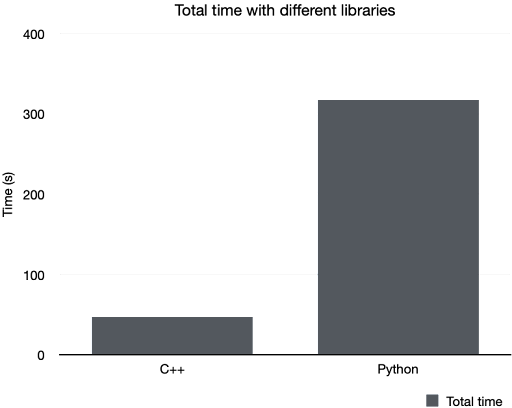
\includegraphics[scale=0.62]{scikit-total.png}
	\caption{Python total runtime using scikit-image to blur 79 images}
	\label{figure:scikit-total}
\end{figure}

Another factor that influences the runtime of a program is how the libraries are linked. The compilation of C++ involves three steps. First is preprocessing, which handles the preprocessor directives, such as “\#include” and “\#define” and, explained simply, replaces them with the content of the respective files. The next step is compilation, which takes the preprocessor’s output and produces an object file. The last step is linking. The linker takes the object files produced by the compiler and produces either a library or an executable file \cite{linking}. Linking can take two different forms. For one, static linking is the process of copying all library modules used in the program into the final executable image. Dynamic (or shared) linking adds the names of the libraries in the executable and then links them at runtime. Programs that use statically linked libraries are usually faster than those using shared libraries. When looking at the profile for C++, dyld was shown as taking up a lot of the total runtime. Dyld is a macOS pre-linking of dynamic libraries. Chandler Caruth, a principal software developer at Google, mused in a Twitter feed about the general slow runtime of a program on macOS as compared to Linux and found that it was due to spending a vast amount of time on dyld \cite{twitter}. This matches what we observed with the xctrace profiler CPU counter.
Of course, the programming language also plays a role in program optimisation. We already saw from previous research that the programming language can influence the runtime for a specific algorithm. Lack of knowledge of the language can cause it to be written in a way that delays the runtime. Additionally, in real-life programming, programmers hardly ever write the entirety program themselves; they use external libraries, packages or models. Choosing the wrong library for our configuration can lead to significant delays, as we have proved in this study. Therefore, choosing a language for a project might be based on available libraries but should also be chosen on the characteristics of the language and if they are optimised for the project. In conclusion, we can say that every program needs its own particular configuration of hardware, OS, language, compilation, external libraries and whichever other factors might contribute.
